% Chapter Template

\chapter{Topical n-grams model} % Main chapter title

\label{topicalngram} % Change X to a consecutive number; for referencing this chapter elsewhere, use \ref{ChapterX}

\lhead{Chapter 5. \emph{Topical n-grams model}} % Change X to a consecutive number; this is for the header on each page - perhaps a shortened title

%----------------------------------------------------------------------------------------
%	Introduction
%----------------------------------------------------------------------------------------

Joint sentiment and topic models have been used to tackle this classification problem. Despite having a hierarchical structure, these generative models have
a bag of words assumption. Due to this fact, they tend to misclassify texts having sentiment in the form of phrases. \textit{LDA} and it's extensions don't 
work properly with phrases. To tackle this situation, we propose an unsupervised approach to sentiment analysis using the topical n-grams model which has been
shown to be effective with phrases. We train the topical n-grams model using three topics i.e., positive, negative, and objective, list of positive and negative
words, and rules to detect positive and negative phrases. New documents are then classified using this trained model. The system gives better results than the 
existing Joint Sentiment Topic model. We also propose an approach to generate a list of positive and negative words using LDA based on our observations reported in~\cref{experiments}.

\section{Introduction}

LDA (Latent Dirichlet Allocation) as shown by \citep*{blei2003latent} is a generative model used to discover topics in a document collection. It gives two 
types of distributions as output, document-topic and word-topic distributions. The document-topic distribution gives the proportion of topics in each document
and the word-topic distribution gives the probability of a word being in each topic. LDA works on the principle of co-occurrence. It assumes that words tending
to appear together belong to the same topic. JST (Joint Sentiment Topic) as explained by \citep*{lin2009joint} is a probabilistic generative model which extends
LDA and discovers both sentiment and topic simultaneously in a document collection. JST has shown promising results on binary sentiment classification. 

There are many extensions of the basic LDA model which try to combine both sentiment and topic to solve the problem of sentiment analysis. All these models 
including LDA have one underlying assumption which makes them unsuitable for text classification purposes. They assume that each word is generated separately 
and independent of other words. This is essentially the bag of words assumption. However, text being a sequence of words, the correct meaning of the text cannot 
be understood by merely capturing co-occurrences. In addition to this, we also need to consider collocation of words. A phrase is a collocation of words which 
usually has more meaning than the individual words making up that phrase. There is a subtle difference between a phrase and collocation of words. Not all collocations
of words can be considered as a phrase. We need a model which takes into account phrases to completely understand the meaning of the text.

Topical n-grams model proposed by \citep*{wang2007topical} is one such generative model which takes into account not only co-occurrences but also collocations of 
words. It also decides whether a particular collocation of words should be considered as a phrase or not. We train this model using 3 topics viz. positive, negative
and objective, using a prior list of positive and negative words, and some rules to identify the subjective nature of phrases. The phrases in our experiments are 
restricted to bigrams. We then use this trained model to infer the topic distribution for new documents. The topic having higher proportion is considered to be the 
class of the document.

In the next section, we will go through some of the related work in this area.

\section{Related Work}

There are many supervised, semi-supervised and unsupervised approaches to solve the sentiment analysis problem. One supervised method based on n-gram analysis is 
explained by \citep*{bespalov2011sentiment}. In this they map the n-grams to a low-dimensional latent semantic space where a classification function can be defined.
Our approach being unsupervised, we will go through some of the related work in that direction. One more motivation to consider only semi-supervised and unsupervised
approaches is the fact that they don't need any corpus and don't have any domain specific limitations. Rule based systems can also be considered as unsupervised 
systems but usually due to exceptions to these rules, their performance is affected. Due to this, we are not considering them in further discussion.

\citep*{turney2002thumbs} used an unsupervised learning algorithm based on mutual information between document phrases and a small set of positive/negative paradigm 
words called seed words to classify the semantic orientation at the word/phrase level. Another unsupervised approach to classify the text at document level was proposed
by \citep*{turney2002unsupervised}. \citep*{eguchi2006sentiment} created a generative model that jointly models sentiment words, topic words and sentiment polarity 
in a sentence as a triple. \citep*{mei2007topic} proposed another generative model, called TSM (Topic Sentiment Mixture) model which can be used to discover topics 
in blogs as well as their associated sentiments. A novel generation model that unifies topic-relevance and opinion generation by a quadratic combination was proposed 
by \citep*{zhang2008generation}. A probabilistic generative model based on LDA called JST (Joint Sentiment Topic) model was shown to perform well for sentiment analysis 
of reviews by \citep*{lin2009joint}. It is a fully unsupervised method and shows good result when priors are used for training. Another extension of LDA which tries
to unify aspect and sentiment was proposed by \citep*{jo2011aspect}. All the unsupervised methods using generative models discussed here operate at the word level. 
Due to this they lose out on the information provided by phrases which may lead to incorrect classification.

In the next section, we will discuss the topical n-gram model in detail.

\section{Topical n-grams model}

n-gram phrases (or collocations) are fundamentally important in many areas of natural language processing (e.g., parsing, machine translation and information retrieval). 
Phrase as the whole carries more information than the sum of its individual components, thus it is much more crucial in determining the topics of document collections 
than individual words \citep*{wang2005note}. However, most of the topic models assume that words are generated independently to each other, i.e., under the bag of words
assumption. The possible over complicacy caused by introducing phrases makes these topic models completely ignore them. It is true that these models with the bag of words
assumption have enjoyed a big success, and attracted a lot of interests from researchers with different backgrounds. A topic model considering phrases would be more 
useful in certain applications. Topical n-grams model is one such generative model. It's generative process is explained as follows,

\begin{enumerate}
 \item Draw multinomial \(\phi_z\) from a Dirichlet prior \(\beta\);
 \item Draw binomial \(\psi_z\) from a Beta prior \(\gamma\);
 \item Draw multinomial \(\sigma_{zw}\) from a Dirichlet prior \(\delta\);
 \item For each document d, draw a multinomial \(θ^{(d)}\) from a Dirichlet prior \(\alpha\); then for each word \({w_i}^{(d)}\) in document \(d\),
    \begin{enumerate}
     \item Draw \({x_i}^{(d)}\) from binomial \(\psi_{{w_{i-1}}^{(d)}}\);
     \item Draw \({z_i}^{(d)}\) from multinomial \(\theta_{(d)}\);
     \item Draw \({w_i}^{(d)}\) from multinomial \(\sigma_{{w_{i-1}}^{(d)}}\) if \({x_i}^{(d)} = 1\); else draw \({w_i}^{d}\) from multinomial \(\phi_{{z_i}^{(d)}}\).
    \end{enumerate}
\end{enumerate}

The main point to infer from this generative process is that the topic assignments for the two terms in a bigram are not required to be identical. In the description of
topic n-grams given in \citep*{wang2005note}, they have used the topic of the last term as the topic of the phrase. But in our experiments, we have used certain rules
as prior information to assign topics to a phrase initially.


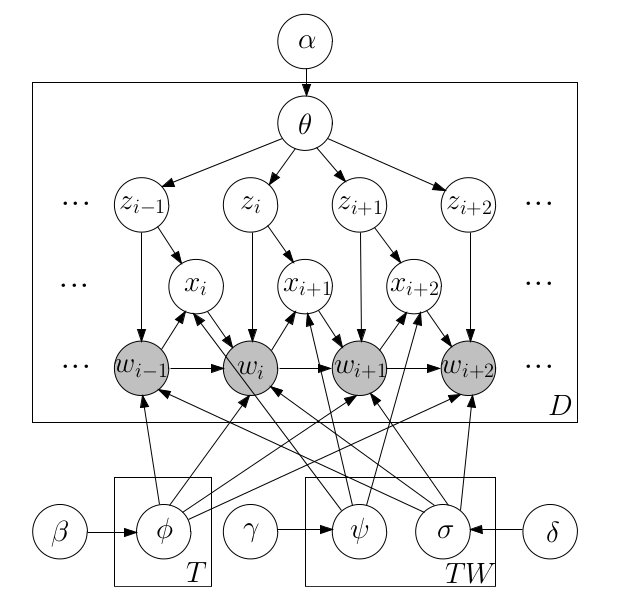
\includegraphics[width=\textwidth]{topicalngram.png} 
\begin{center}
 Figure 5.1 Topical n-grams model
\end{center}

\subsection{Inferencing}

Gibbs sampling is used to conduct approximate inference in this paper. During Gibbs sampling, we draw the topic assignment \(z_i\) and the bigram status \(x_i\) 
iteratively for each word \(w_i\) according to the following conditional probability distribution:

\begin{equation}
p(z_i,x_i | z_{-i},w_{-i},w,\alpha,\beta,\gamma,\delta) \propto
\frac{\gamma_{x_i} + p_{z_{i-1}w_{i-1}x_i}}{\sum_{k=0}^1 {(\gamma_k+p_{z_{i-1}}w_{i-1}k)}} {(\alpha_{z_i} + q_{d_{z_i}})} \times \left\{ 
  \begin{array}{l l}
    \frac{\beta_{w_i} + n_{z_i w_i}}{\sum_{v=1}^V {(\beta_v+n_{z_i v})}} & \quad \text{if $x_i$ is even}\\
    \frac{\delta_{w_i} + m_{z_i w_{i-1} w_i}}{\sum_{v=1}^V {(\delta_v + m_{z_i w_{i-1} v})} } & \quad \text{if $n$ is odd}
  \end{array} \right.
\end{equation}

where, 

\(z_{-i}\) denotes the topic assignments for all word tokens except word \(w_i\), \\ 
\(x_{-i}\) represents the bigram status for all tokens except word \(w_i\), \\ 
\(n_{zw}\) represents how many times word \(w\) is assigned into topic \(z\) as a unigram, \\
\(m_{zwv}\) represents how many tmes word \(v\) is assigned as the second term of a bigram given the previous word \(w\), \\
\(p_{zwk}\) denotes how many times the status variable \(x\) equals \(k\) given the previous word \(w\) and previous word's topic \(z\), and \\
\(q_{dz}\) represents how many times a word is assigned to topic \(z\) in document d.

In next section, we will explain the use of topical n-grams model for sentiment analysis

\section{Topical n-grams model for Sentiment Analysis}

To make use of topical n-grams model for sentiment classification, we use an approach similar to using LDA for sentiment classification.

\begin{itemize}
 \itemsep0em
 \item Set number of topics equal to 3.
 \item Remove stop-words.
 \item Remove objective words as they won't affect sentiment. The objective words in this case do not include the negation words like \textit{doesn't, 
 won't, no}, etc. This is to ensure that we can catch negation of polarity when they are used with subjective words.
 \item Apply Gibbs Sampling with prior. The prior used in this case is more sophisticated and can handle both words and phrases. In case of words, if 
 is not present in a bigram then simply use a list of positive and negative words to assign positive or negative topic. If the word is present in a 
 bigram then assign it the objective topic. There are some rules to detect and assign topics to phrases which are explained next.
 \item Use the trained model to classify a new document as positive or negative. Here, we ignore the proportion of the objective topic.
\end{itemize}

\subsubsection*{Rules for Topic assignment of phrases}

At present, our rules are restricted to bigrams. We plan to extend them as explained in Section~\cref{conclusions}.
In the following rules, we mean topic when we say polarity. The use of polarity makes it easy to understand
the rules as they are concerned with subjectivity.

\begin{enumerate}
 \itemsep0em
 \item If the first word in the bigram is a negation word and the second word is subjective then the polarity
 of the bigram is opposite to the polarity of the second word. \\
 \textbf{Examples:} \textit{won't like, won't regret, etc.}. Here, \textit{won't like} is assigned negative
 polarity and \textit{won't regret} is assigned positive polarity.
 \item If both the words in the bigram are subjective then are two cases. If both words are of the same polarity
 then resultant polarity is the same. But if their polarities are different, then the polarity of the first word
 is assigned to the bigram. \\
 \textbf{Examples:} \textit{beautifully amazing} is positive as both words as positive. \textit{lack respect} is
 assigned negative as per the rules.
\end{enumerate}

One salient feature of this approach is that it is an unsupervised method and can work on any domain. 

\section*{SUMMARY}

In this chapter, we dicussed the motivation behind the topical n-grams model. Later on, we discussed the inference equation used by it. At the end,
we proposed an approach to use this model for sentiment analysis. The experiments and results obtained are discussed in ~\cref{experiments}.

In the next chapter, we will show the use of deep semantics for sentiement analysis.